\documentclass[a4paper, 10pt]{article}

%PACOTES
\usepackage[lmargin=2.5cm, rmargin=2.5cm, tmargin=2.5cm, bmargin=2.5cm ]{geometry}
\usepackage[utf8]{inputenc}
\usepackage[T1]{fontenc}
\usepackage[brazil]{babel}
\usepackage[style=ieee]{biblatex}
\usepackage{graphicx}
\usepackage{amsmath}
\usepackage{amsfonts}
\usepackage{amssymb}
\usepackage{changepage}
\usepackage{verbatim}
\usepackage{float}
\usepackage{csquotes}
\usepackage{caption}
\usepackage{subcaption}
\usepackage{biblatex}
\usepackage[nottoc,numbib]{tocbibind}
\usepackage{blindtext}
\usepackage{geometry}
\usepackage{array,booktabs}
\usepackage{indentfirst}
\usepackage{ragged2e}
\usepackage{slashbox}

\newcolumntype{P}[1]{>{\centering\arraybackslash}p{#1}}

\setlength{\parskip}{6pt}

\graphicspath{ {images/} }

\addbibresource{bibliography.bib}

\begin{document}
% Capa
\thispagestyle{empty}

\begin{figure}[!ht]
	\centering
	\begin{subfigure}[b]{0.3\textwidth}
         \centering
         
\includegraphics[width=\textwidth]{Horizontal Vermelho - Logotipo CIn-UFPE.png}
     \end{subfigure}
     \begin{subfigure}[b]{0.3\textwidth}
         \centering
         
\includegraphics[width=\textwidth]{logo_ufpe.png}
     \end{subfigure}
\end{figure}

\Large\begin{center}
    {\textsc{Universidade Federal de Pernambuco \\ Centro de Informática}}
\end{center}

\vspace{4cm}
\begin{center}
	\huge{\textsc{\textbf{
	    Implementação do método de geração das malhas de baixa resolução para a simulação multiescala de reservatórios de petróleo em três dimensões
	}}}
\end{center}
\vspace{5cm}

\begin{center}
    \textbf{Aluno:} Filipe Antônio Cumaru Silva Alves (facsa@cin.ufpe.br)
\end{center}
\begin{center}
    \textbf{Orientador:} Prof. Dr. Paulo Roberto Maciel Lyra (paulo.lyra@ufpe.br)
\end{center}
\begin{center}
    \textbf{Área:} Métodos Numéricos Computacionais
\end{center}

\vspace{2cm}
\begin{center}
    {Recife, 15 de outubro de 2021}
\end{center}

\clearpage
\setcounter{page}{1}

\fontsize{11}{13.2}\selectfont
% ----------------------------

% Sumário
\tableofcontents

\thispagestyle{empty}

\newpage

% ----------------------------
\section{Resumo}

\noindent
A simulação de reservatórios de petróleo é uma tarefa desafiadora por envolver fenômenos em múltiplas escalas e pela dificuldade em balancear o detalhamento do modelo discreto da descrição do reservatório, denominado malha, com o tempo de computação necessário para realização da simulação. Neste contexto, métodos multiescala são usados afim de efetuar a simulação numa discretização de menor resolução mas ainda capaz de preservar aspectos importantes da física do reservatório. Uma etapa importante é a geração de tal modelo de menor resolução, principalmente para casos tridimensionais. Neste trabalho, será implementada uma estratégia para geração de malhas voltadas para simulação multiescala 3D de reservatórios de petróleo. O programa será desenvolvido na linguagem Python com auxílio de bibliotecas de computação científica e os resultados serão verificados utilizando-os como entrada para métodos numéricos disponíveis na literatura e desenvolvidos no grupo de pesquisa do professor orientador.

% ----------------------------
\clearpage
% ----------------------------
\section{Contexto}

A simulação numérica do escoamento de fluidos em reservatórios de petróleo tem sido utilizada há décadas pela indústria afim de prever taxas de produção de óleo e o comportamento do reservatório ao longo da exploração, permitindo a redução de custos e melhora na eficiência de extração. Apesar de bastante estudada, a simulação de reservatórios ainda é uma atividade desafiadora do ponto de vista computacional devido à complexidade dos modelos matemáticos usados e à escala em que são conduzidos os experimentos.

A realização da simulação passa pela solução de um modelo matemático. No contexto do estudo do escoamento de fluidos em meios porosos, os modelos matemáticos envolvem equações diferenciais parciais não lineares com variáveis espaciais em uma, duas ou três dimensões além de uma variável temporal. Exemplos de modelos usados são as equações de Navier-Stokes, a lei de Darcy e as equações de Stokes-Brinkman. Na ampla parte dos casos, não é possível obter uma solução analítica para estas equações e métodos numéricos são aplicados para obter uma solução aproximada.

Os métodos de diferenças finitas, elementos finitos e volumes finitos são aqueles mais utilizados para aproximação da solução do escoamento no espaço. Para estes esquemas, é necessária uma discretização do meio conhecida como malha. Assim, quanto maior for a resolução da malha, isto é, quanto maior o número de subdivisões na discretização, maior a acurácia da solução. Entretanto, a alta resolução gera maior complexidade de simulação e demanda mais recursos computacionais. Atualmente, modelos com número de elementos da ordem de $10^8$ já foram publicados, a exemplo do modelo de bilhões de elementos simulado pela IBM \cite{IBMBillion}. Uma simulação desta magnitude é difícil de ser praticada em \textit{softwares} comerciais disponíveis ao público.

A necessidade de incorporar informações da malha de alta resolução na malha dos simuladores tradicionais, de baixa resolução, deu origem às técnicas de transferência de escala. Entre elas, destacam-se dois tipos: métodos \textit{upscaling} e métodos multiescala. Os primeiros utilizam algum tipo de homogeneização para projetar uma propriedade física da escala mais refinada na menos refinada, onde a simulação é então realizada. Já a segunda técnica deriva uma série de operadores algébricos que projetam o sistema de equações construído no espaço da malha de alta resolução no espaço da malha de baixa resolução. O sistema de equações é resolvido nesta escala e, diferentemente do método \textit{upscaling}, a resposta é projetada de volta na malha de alta resolução. Isto preserva o acoplamento natural entre escalas, diminuindo problemas com inconsistências e perdas de informação intrínsecas aos métodos \textit{upscaling}, como visto em Hou e Wu \cite{HouAndWu}, Jenny et al. \cite{JennyAndLeeAndTchelepi}, e Zhou e Tchelepi \cite{ZhouAndTchelepi}.

Um passo fundamental para a aplicação dos métodos multiescala é a construção da malha de menor resolução em que será feita a simulação. Tais algoritmos de pré-processamento são definidos de acordo com a formulação do método multiescala de solução. Contudo, para o caso 3D, poucas estratégias estão disponíveis, sendo possível citar o trabalho de M\o yner \cite{Olav} neste sentido. Assim, neste trabalho será implementada uma extensão do método para a geração das malhas na escala de baixa resolução apoiado no conceito de \textit{background grid} proposto por Souza et al. \cite{Souza} para malhas tridimensionais.

% ----------------------------
\clearpage
% ----------------------------
\section{Objetivos}

\subsection{Objetivos gerais}

Implementar o método para geração das malhas de menor resolução apoiado no conceito de \textit{background grid} aplicado à simulação multiescala em três dimensões de reservatórios de petróleo.

\subsection{Objetivos específicos}

São objetivos específicos deste trabalho:

\begin{itemize}
    \item Estender o método de geração das malhas na escala de menor resolução apoiado no conceito de \textit{background grid} para três dimensões;
    \item Estudar algoritmos para detecção de interseção entre geometrias diversas; e
    \item Avaliar a qualidade das malhas geradas aplicando-as na simulação com métodos multiescala já existentes.
\end{itemize}

% ----------------------------
\clearpage
% ----------------------------
\section{Metodologia}

O trabalho proposto será desenvolvido em três etapas: estudo de métodos multiescala em três dimensões e revisão de algoritmos de geometria computacional; implementação e testes da estratégia definida; e avaliação dos resultados e escrita da monografia.

Primeiramente, será feita uma revisão da definição do método \textit{background grid} em duas dimensões para sua expansão para reservatórios tridimensionais. Para esta tarefa, também será necessário o estudo da teoria de métodos multiescala, bem como uma revisão bibliográfica de algoritmos de geometria computacional devido à alta demanda de operações envolvendo cálculos de interseções entre formas diversas. Ao fim desta etapa, a formulação do método em três dimensões será obtida bem como os requisitos para sua implementação.

Na etapa seguinte, será implementada a formulação definida em linguagem Python com auxílio das bibliotecas Numpy \cite{Numpy}, Scipy \cite{Scipy} e IMPRESS \cite{Impress}, esta última baseada numa implementação da biblioteca MOAB \cite{MoabReport, MoabPaper} que permite a manipulação e extração de informações de malhas diversas.

Por fim, a implementação produzida será verificada por meio da sua aplicação a métodos multiescala 3D disponíveis na literatura, notavelmente a formulação de M\o yner \cite{Olav} e Souza et al. \cite{Souza}.

% ----------------------------
\clearpage
% ----------------------------
\section{Cronograma de trabalho}

\centering
{\def\arraystretch{2}\tabcolsep=10pt
\begin{tabular}{@{}P{5cm}||c|c|c|c}
    \backslashbox[4.5cm]{Atividade}{Mês} & Setembro & Outubro & Novembro & Dezembro \\
    \hline
    \hline
    Estudo do algoritmo para agrupamento de volumes da malha grossa & X & & &  \\
    \hline
    Implementação de estratégias de detecção de interseções entre geometrias & X & X & &  \\
    \hline
    Implementação do método de construção de conectividades entre volumes na malha grossa & & X & X &  \\
    \hline
    Geração e avaliação dos resultados & & & X & X \\
    \hline
    Redação do relatório final & & & X & X  \\
\end{tabular}}

% ----------------------------
\clearpage
% ----------------------------
\raggedright
\section{Possíveis avaliadores}

Como possível avaliador sugerimos o Prof. Dr. Odilon Maroja da Costa Pereira Filho.

% ----------------------------
\clearpage
% ----------------------------
\raggedright
\section{Assinaturas}

\vspace{3cm}

\begin{figure}[!htb]
    \centering
    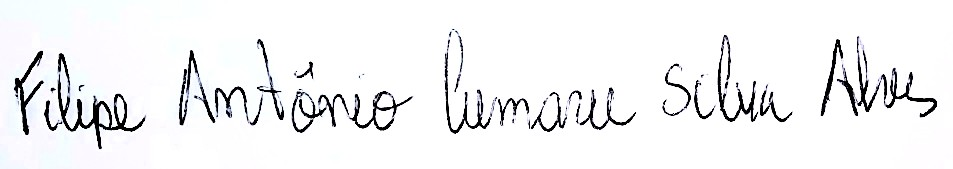
\includegraphics[scale=0.25]{assinatura.jpg}
    \label{fig:my_label}
\end{figure}

\centering
\begin{tabular}{@{}P{1.3cm}P{10cm}@{}}
& \hrulefill \\[0.5cm]
& Filipe Antônio Cumaru Silva Alves \\[0.25cm]
& \textbf{Orientando} \\
\end{tabular}

\vspace{3cm}

\centering
\begin{tabular}{@{}P{1.3cm}P{10cm}@{}}
& \hrulefill \\[0.5cm]
& Paulo Roberto Maciel Lyra \\[0.25cm]
& \textbf{Orientador} \\
\end{tabular}

% ----------------------------

\clearpage

\raggedright
\addcontentsline{toc}{section}{Referências}
\printbibliography

\end{document}

	